\documentclass[a4paper,12pt]{article}
\usepackage[latin1]{inputenc}
\usepackage[spanish]{babel}
\usepackage{graphicx}
\usepackage{amsmath}
\usepackage{wrapfig}
\setlength{\textheight}{250mm}
\setlength{\textwidth}{165mm}
\setlength{\topmargin}{-15mm}
\setlength{\oddsidemargin}{0pt}
\pagestyle{empty}

\begin{document}

\def\bm#1{{\mbox{\boldmath $#1$}}}
\def\eqdef{\buildrel \rm def \over =}
\def\signo{\mathop{\rm signo}\nolimits}

\mbox{}\vspace*{-20mm}

{\centering
{\small\sc Escuela T�cnica Superior de Ingenieros de Caminos, Canales y Puertos (Madrid)}\\*[4mm]
{\Large\bf M�todo de los Elementos Finitos}\\*[4mm]
Pr�ctica 8. Tecnolog�a de elementos / Elasticidad 3D. \\*[4mm]
}

% \vspace{4mm}

\noindent
Se considera una l�mina cil�ndrica de radio medio $R=300$,
longitud $L=600$ y espesor $t=3$, cuyo material es el�stico lineal con
propiedades mec�nicas $E=300$ y $\nu=0.3$. En los extremos del cilindro hay
dos diafragmas r�gidos circulares, y en dos puntos diametralmente
opuestos de la secci�n transversal media est�n aplicadas sendas cargas radiales
de compresi�n de valor $P=1.0$ cada una de ellas. Este es un ejemplo cl�sico
del an�lisis de l�minas, que en esta pr�ctica se analiza con elementos s�lidos
tridimensionales. Para la discretizaci�n se tendr�n en cuenta las condiciones de
simetr�a existentes, y se utilizar�n discretizaciones de $8 \times 8$,
$16 \times 16$, $32 \times 32$ y $64 \times 64$ elementos en direcci�n
meridional y circunferencial, y $1$, $3$ y $5$ elementos en el espesor. Las
formulaciones a considerar son hexaedros de $8$ nodos con fomulaci�n est�ndar en
desplazamientos, con formulaci�n mixta y con modos incompatibles.

Obtener el desplazamiento radial en el puntos en que est� aplicada la carga,
comparando este valor con el de referencia: $u_A=0.18248$

\begin{center}
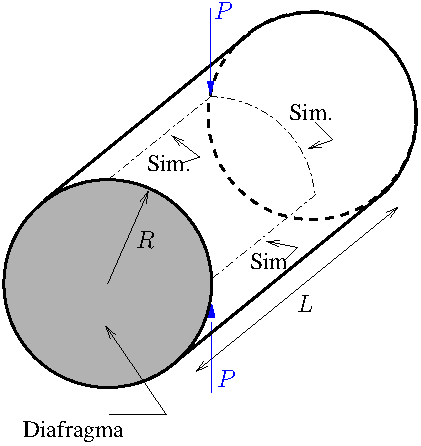
\includegraphics[width=0.45\textwidth]{pinched}
\end{center}
\end{document}
